\documentclass[12pt]{article}
\usepackage{amsmath}
\usepackage{amsthm}
\usepackage{amsfonts}
\usepackage{amssymb}
\usepackage{enumerate}
\usepackage{tikz}
\usepackage{pgfplots}
\pgfplotsset{compat=1.18}
\usepackage[margin = .75in]{geometry}
\definecolor{purple}{RGB}{51,0,111} % Official UW color scheme
\usepackage[colorlinks=true, allcolors=purple]{hyperref} %% For links
\pagestyle{empty} %% Gets rid of the page number
%% New Commands
%% For our common number systems.
\newcommand{\Nn}{\mathbb{N}}
\newcommand{\Zz}{\mathbb{Z}}
\newcommand{\Qq}{\mathbb{Q}}
\newcommand{\Rr}{\mathbb{R}}
\newcommand\set[1]{\{ #1 \}} %%\set{abc} ==> {abc}
\newcommand\abs[1]{\left| #1 \right|} %% \abs{abc} ==> |abc|
\newcommand\parens[1]{\left( #1 \right)}
\newcommand\brac[1]{\left[ #1 \right]}
\newenvironment{solution}
  {\renewcommand\qedsymbol{$\blacksquare$}\begin{proof}[Solution]}
  {\end{proof}}


\begin{document}
\raggedright
\begin{center}
      {\large Math 1512 Calculus 1 Review}\\
  {Fall 2026}\\

\end{center}


\begin{enumerate}
\item Formulas to know.
    \begin{enumerate}
        \item The definition of ``$f$ is continuous at $x=a$''
        \item $f'(a)$, the derivative of $f$ at $x=a$, written as a limit in two ways (as $x \to a$ and as $h \to 0$)
        \item $\lim_{\theta \to 0} \frac{\sin \theta}{\theta}$ and $\lim_{\theta \to 0} \frac{\cos \theta - 1}{\theta}$
        \item Derivatives of $\sin(x)$, $\cos(x)$, $\tan(x)$, $\sec(x)$, $\csc(x)$, $\cot(x)$
        \item Power rule, product rule, quotient rule, chain rule
        \item The linearization $L(x)$ of $f$ at $x=a$, and the differential $dy$
        \item Definition of a critical number of $f$
        \item State the Intermediate Value Theorem, the Extreme Value Theorem, Fermat's Theorem, and the Mean Value Theorem
        \item First derivative test, second derivative test, and the definition of an inflection point
        \item Antiderivatives of $x^n$ ($n \neq -1$), $\sin(x)$, $\cos(x)$, $\sec^2(x)$, $\sec(x)\tan(x)$
        \item The definite integral $\int_a^b f(x) dx$ as a limit of Riemann sums
        \item Both parts of the Fundamental Theorem of Calculus
        \item The average value of $f$ on $[a,b]$
        \item Volume of a cylinder, a cone, and a sphere. Area of a circle. Surface area of a sphere.
    \end{enumerate}

    \newpage

\item Limits from a graph. Let $g$ be the function graphed below. A filled dot is a point on the graph, an open dot is not.

\begin{center}
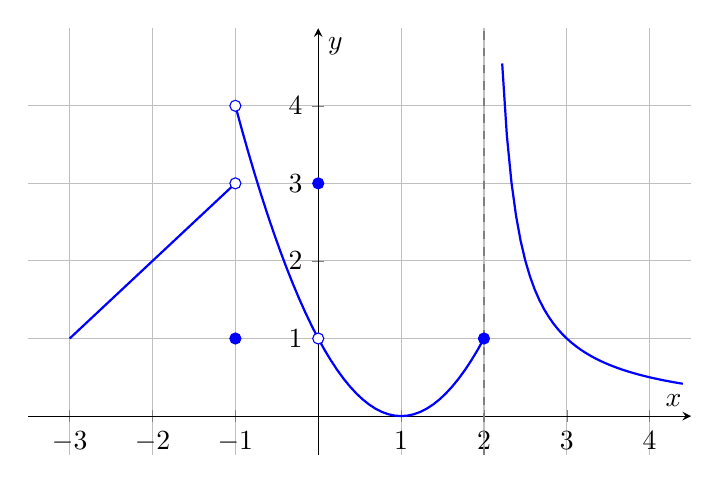
\begin{tikzpicture}
\begin{axis}[width=10cm, height=7cm, xmin=-3.5, xmax=4.5, ymin=-0.5, ymax=5, axis lines=middle, grid=major, xtick={-3,...,4}, ytick={0,...,4}, xlabel={$x$}, ylabel={$y$}]
    \addplot[blue, thick, domain=-3:-1]{x+4};
    \addplot[blue, thick, domain=-1:2, samples=40]{(x-1)^2};
    \addplot[blue, thick, domain=2.22:4.4, samples=40]{1/(x-2)};
    \addplot[blue, only marks, mark=*, fill=white] coordinates {(-1,3) (-1,4) (0,1)};
    \addplot[blue, only marks, mark=*] coordinates {(-1,1) (0,3) (2,1)};
    \addplot[gray, dashed] coordinates {(2,-0.5) (2,5)};
\end{axis}
\end{tikzpicture}
\end{center}

    \begin{enumerate}
        \item $g(-1)$, $\lim_{x \to -1^-} g(x)$, $\lim_{x \to -1^+} g(x)$, $\lim_{x \to -1} g(x)$
        \item $g(0)$ and $\lim_{x \to 0} g(x)$
        \item $\lim_{x \to 2^-} g(x)$, $\lim_{x \to 2^+} g(x)$, $\lim_{x \to 2} g(x)$
        \item At which $x$ values in $(-3,4)$ is $g$ not continuous? For each, say whether the discontinuity is removable, a jump, or infinite.
        \item At which of these $x$ values is $g$ continuous from the left? From the right?
        \item Suppose $\lim_{x \to a} f(x) = 4$ and $\lim_{x \to a} h(x) = -2$. Use the limit laws to evaluate $\lim_{x \to a} [3f(x) - 5h(x)]$, $\lim_{x \to a} f(x)h(x)$, $\lim_{x \to a} \frac{f(x)}{h(x)}$, and $\lim_{x \to a} \parens{\sqrt{f(x)} + h(x)^2}$.
    \end{enumerate}

    \newpage


\item Computing limits. Evaluate the limit, or explain why it does not exist. Use $\infty$ or $-\infty$ when appropriate.
    \begin{enumerate}
        \item $\lim_{x \to 3} \frac{x^2-2x-3}{x^2-9}$
        \item $\lim_{x \to 5} \frac{\sqrt{x+4}-3}{x-5}$
        \item $\lim_{x \to -1} \frac{\frac{1}{x+3} - \frac{1}{2}}{x+1}$
        \item $\lim_{x \to 4} \frac{5}{x^2-3x-4}$ (consider the one-sided limits)
        \item $\lim_{x \to -1} \frac{x}{(x+1)^2}$
        \item $\lim_{x \to 2} \frac{x^2-4}{\abs{x-2}}$
    \end{enumerate}

\item Squeeze Theorem.
    \begin{enumerate}
        \item $\lim_{x \to 0} x^2 \sin\parens{\frac{3}{x}}$
        \item If $2x - 1 \leq f(x) \leq x^2 - 2x + 3$ for all $x$, find $\lim_{x \to 2} f(x)$.
        \item Explain why the product law cannot be used to evaluate the limit in (a).
    \end{enumerate}

    \newpage

\item Limits at infinity and asymptotes.
    \begin{enumerate}
        \item $\lim_{x \to \infty} \frac{3x^2-x+2}{5x^2+4}$
        \item $\lim_{x \to -\infty} \frac{\sqrt{4x^2+1}}{x+3}$ (Recall $\sqrt{x^2} = \abs{x}$)
        \item $\lim_{x \to \infty} \parens{\sqrt{x^2+6x} - x}$
        \item Find all vertical and horizontal asymptotes of $f(x) = \frac{2x^2-2}{x^2+x-2}$. Why is $x=1$ not a vertical asymptote?
    \end{enumerate}

\item Continuity and the Intermediate Value Theorem.
    \begin{enumerate}
        \item For each property, sketch the graph of a function $f$ defined on $[0,4]$ with that property, and name the type of discontinuity at $x=2$. (i) $\lim_{x \to 2} f(x) = 3$ but $f(2) = 1$. (ii) $\lim_{x \to 2^-} f(x) = 1$ and $\lim_{x \to 2^+} f(x) = 4$. (iii) $\lim_{x \to 2^+} f(x) = -\infty$.
        \item Let $f(x) = \begin{cases} x+2 & x < -1 \\ x^2 & -1 \leq x \leq 1 \\ 3-x & x > 1 \end{cases}$. Sketch the graph of $f$. Use the definition of continuity to decide whether $f$ is continuous at $x=-1$ and at $x=1$. At which $x$ values is $f$ not differentiable?
        \item Where is $g(x) = \frac{\sqrt{x-3}}{x^2-25}$ continuous?
        \item Find $a$ and $b$ so that $f(x) = \begin{cases} 2 & x < 1 \\ ax + b & 1 \leq x < 4 \\ 8 & x \geq 4 \end{cases}$ is continuous everywhere.
        \item Show that $x^3 + x - 1 = 0$ has a solution in $(0,1)$.
    \end{enumerate}

    \newpage

\item The derivative as a limit.
    \begin{enumerate}
        \item Let $f(x) = x^3$ and $P = (2,8)$. Write the slope of the secant line through $P$ and $Q = (x, x^3)$. Take the limit as $x \to 2$ to find the slope of the tangent line at $P$, then write the tangent line. Sketch the curve, $P$, one secant line, and the tangent line.
        \item Compute $f'(x)$ directly from $f'(x) = \lim_{h \to 0} \frac{f(x+h)-f(x)}{h}$ for $f(x) = \frac{x}{x+2}$.
        \item Compute $f'(x)$ from the same limit for $f(x) = \sqrt{2x+1}$. Then find the tangent line at $(4,3)$.
        \item A ball's height is $h(t) = 200 - 16t^2$ feet after $t$ seconds. Find the slope of the secant line between $t=1$ and $t=3$, with units. Then find the instantaneous velocity at $t=2$ as a limit.
        \item Show that $f(x) = \sqrt[3]{x}$ is continuous at $x=0$ but not differentiable there. What does the tangent line at $x=0$ look like?
        \item Each limit is $f'(a)$ for some function $f$ and number $a$. Find $f$ and $a$, then evaluate: $\lim_{h \to 0} \frac{(2+h)^4 - 16}{h}$ and $\lim_{x \to \pi/2} \frac{\cos x}{x - \frac{\pi}{2}}$.
        \item Sketch the graph of $f'$ for the function $f$ graphed below. Where is $f'$ zero, positive, negative?

\begin{center}
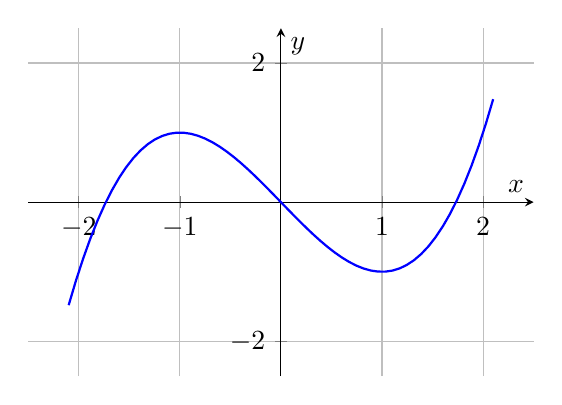
\begin{tikzpicture}
\begin{axis}[width=8cm, height=6cm, xmin=-2.5, xmax=2.5, ymin=-2.5, ymax=2.5, axis lines=middle, grid=major, xlabel={$x$}, ylabel={$y$}]
    \addplot[blue, thick, domain=-2.1:2.1, samples=60]{(x^3-3*x)/2};
\end{axis}
\end{tikzpicture}
\end{center}
    \end{enumerate}

    \newpage

\item Differentiation rules. Differentiate, using the power, product, and quotient rules.
    \begin{enumerate}
        \item Find $f'(x)$ if $f(x) = 6x^4 - \frac{2}{x^2} + 3\sqrt[3]{x} - 7$
        \item Find $g'(x)$ if $g(x) = (x^3+2x)(4-x^2)$
        \item Find $y'$ if $y = \frac{x^2+1}{2x+1}$
        \item Find the points on the curve $y = x^3 - 3x^2 - 9x + 2$ where the tangent line is parallel to the line $y = 15x$.
        \item Find the tangent line to $f(x) = x^3 - 4x^2 + 5$ at $x=3$.
        \item A particle has position $s(t) = t^3 - 9t^2 + 24t$ meters at time $t$ seconds. Find the velocity $v(t)$ and acceleration $a(t)$, with units. When is the particle at rest?
    \end{enumerate}

\item Trig derivatives.
    \begin{enumerate}
        \item Starting only from $\frac{d}{dx}\sin x = \cos x$ and $\frac{d}{dx}\cos x = -\sin x$, derive the formula for $\frac{d}{dx}\sec x$. Then find $\frac{d^2}{dx^2}\tan x$.
        \item Evaluate $\lim_{x \to 0} \frac{\sin(4x)}{3x}$ and $\lim_{x \to 0} \frac{1-\cos x}{x\sin x}$.
        \item Find $f'(\theta)$ if $f(\theta) = \theta^2 \cos \theta - 4 \tan \theta$
        \item Find $y'$ if $y = \frac{\sec x}{1 + \tan x}$
        \item Find the tangent line to $y = x\cos x$ at the point $(\pi, -\pi)$.
    \end{enumerate}

    \newpage

\item Chain rule.
    \begin{enumerate}
        \item Use the table to find $(f \circ g)'(1)$, $(g \circ f)'(1)$, and $(fg)'(2)$.
        \[
        \begin{array}{c|cccc}
        x & 0 & 1 & 2 & 3 \\ \hline
        f(x) & 2 & 3 & 0 & 1 \\
        f'(x)& -1 & 4 & 2 & 5 \\
        g(x) & 1 & 2 & 3 & 0 \\
        g'(x)& 3 & -2 & 1 & 4
        \end{array}
        \]
        \item Find the tangent line to $y = \tan(\sqrt{x})$ at $x = \frac{\pi^2}{16}$.
        \item Find the tangent line to $y = (x^2-3)^5$ at $x = 2$.
        \item Find $f'(x)$ if $f(x) = \sqrt{x^4+3x^2+5}$
        \item Find $g'(x)$ if $g(x) = 3x^2 \sec(x^3-1)$
        \item Find $h'(x)$ if $h(x) = \frac{\cos^2(x)}{(2x+3)^3}$
        \item Find $y'$ if $y = \sin\parens{(3x^2-1)^4}$
        \item Find all points $(x,y)$ with $0 \leq x < 2\pi$ where $y = 2\sin x + \cos(2x)$ has a horizontal tangent line.
    \end{enumerate}

\item Implicit differentiation.
    \begin{enumerate}
        \item For the ellipse $x^2 + 4y^2 = 16$, find $\frac{dy}{dx}$ and $\frac{d^2y}{dx^2}$. Simplify $\frac{d^2y}{dx^2}$ using the equation of the ellipse.
        \item Find the tangent line to $\sin(x+y) = 2x - 2y$ at $(\pi, \pi)$.
        \item Find the tangent line to $x^3 + y^3 = 9xy$ at $(2,4)$.
        \item For the curve $y^2 = x^3 - 3x + 2$, find $\frac{dy}{dx}$, the tangent line at $(2,2)$, and all points with a horizontal tangent line.
    \end{enumerate}

    \newpage

\item Related rates. Draw a picture, name the quantities that change, and write the equation relating them before differentiating.
    \begin{enumerate}
        \item A 13 ft ladder leans against a wall. The bottom slides away from the wall at 2 ft/s. How fast is the top sliding down when the bottom is 5 ft from the wall?
        \item A tank is an inverted cone with radius 3 m at the top and height 6 m. Water is pumped in at 4 $\text{m}^3$/min. How fast is the water level rising when the water is 4 m deep?
        \item The height of a cylinder increases at 3 cm/min while its radius decreases at 0.5 cm/min. How fast is the volume $V=\pi r^2 h$ changing when $r=2$ cm and $h=4$ cm? Is it increasing or decreasing?
        \item A 6 ft tall person walks away from a 15 ft lamppost at 3 ft/s. How fast is the tip of the person's shadow moving?
        \item A marble moves along the curve $x^2 + xy + y^2 = 9$ ($x, y$ in feet). At $(3,0)$, $x$ is decreasing at 2 ft/s. Is $y$ increasing or decreasing, and how fast?
    \end{enumerate}

\item Linear approximation and differentials.
    \begin{enumerate}
        \item Find the linearization of $f(x) = \sqrt[3]{x}$ at $a=27$. Use it to approximate $\sqrt[3]{27.27}$.
        \item Find the linearization of $f(x) = \sin x$ at $a = \frac{\pi}{6}$. Use it to approximate $\sin\parens{\frac{\pi}{6} + 0.02}$.
        \item The radius of a sphere is measured as 10 cm with a possible error of 0.05 cm. Use differentials to estimate the maximum error in the computed volume.
    \end{enumerate}

    \newpage

\item Extreme values.
    \begin{enumerate}
        \item Find the critical numbers of $f(x) = x^{2/3}(x-5)$. Which come from $f'(x) = 0$ and which from $f'(x)$ undefined?
        \item[] Find the absolute extrema of $f$ on the given interval.
        \item $f(x) = x^4 - 8x^2 + 3$ on $[-1,3]$
        \item $f(x) = \frac{4x}{x^2+4}$ on $[-4,0]$
        \item $f(x) = x\sqrt{4-x^2}$ on $[-1,2]$
        \item $f(x) = 2\cos x + \sin(2x)$ on $[0, \pi]$
    \end{enumerate}

\item Mean Value Theorem.
    \begin{enumerate}
        \item Find every $c$ guaranteed by the MVT for $f(x) = x^2 - 4x + 1$ on $[1,5]$.
        \item If $f(2) = -1$ and $f'(x) \leq 3$ for all $x$, how large can $f(6)$ be?
        \item Show that $f(x) = \abs{x}$ on $[-1,1]$ has no $c$ with $f'(c) = \frac{f(1)-f(-1)}{1-(-1)}$. Which hypothesis of the MVT fails?
        \item Show that $x^3 + 5x - 2 = 0$ has exactly one real solution.
    \end{enumerate}

    \newpage

\item Shape of a graph. Find the intervals of increase and decrease, the local extrema, the intervals of concavity, and the inflection points.
    \begin{enumerate}
        \item $f(x) = x^3 - 6x^2 + 9x + 1$
        \item $f(x) = 3x^4 - 4x^3$
        \item $f(x) = x + 2\sin x$ on $[0, 2\pi]$
        \item Use the second derivative test to classify the critical numbers of $f(x) = x^4 - 2x^2$.
        \item Sketch a function with $f' > 0$ and $f'' < 0$ everywhere. Sketch one with $f' < 0$ and $f'' > 0$ everywhere.
        \item Find constants $a$ and $b$ so that $f(x) = x^3 + ax^2 + bx$ has an inflection point at $x=1$ and a local minimum at $x=3$. Where is its local maximum?
    \end{enumerate}

\item Curve sketching. Find the domain, intercepts, asymptotes, intervals of increase and decrease, local extrema, concavity, and inflection points. Then sketch the graph and label all of these.
    \begin{enumerate}
        \item $f(x) = \frac{1}{x^2+3}$
        \item $f(x) = \frac{x^2}{x-1}$ (this one has a slant asymptote)
        \item $f(x) = x - 2\sqrt{x}$
    \end{enumerate}

    \newpage

\item Optimization. Draw a picture, introduce variables, write the quantity to optimize as a function of one variable, and verify that your answer is a max or min.
    \begin{enumerate}
        \item A closed box has a rectangular base whose length is twice its width, and its volume is $72\ \text{ft}^3$. Find the dimensions that use the least material.
        \item A closed cylindrical can holds $16\pi\ \text{cm}^3$. Find the radius and height that minimize its surface area.
        \item A rectangle has its base on the $x$-axis and its two upper corners on the semicircle $y = \sqrt{25 - x^2}$. Find the largest possible area.
        \item A rectangular pen is split in half by a divider parallel to one side. The outer fence costs \$4 per meter and the divider costs \$2 per meter. With \$200, what is the largest possible area?
        \item Find the points on the parabola $y = x^2$ closest to the point $(0,2)$.
    \end{enumerate}

\item Antiderivatives and initial value problems. Find the most general antiderivative.
    \begin{enumerate}
        \item $f(x) = 6x^2 - \frac{4}{x^3} + 2\sqrt{x}$
        \item $g(x) = \frac{x^2 - 3x + 2\sqrt{x}}{x}$
        \item $h(t) = 3\cos t - 2\sec^2 t + \sec t \tan t$
        \item If $f'(x) = 3\sqrt{x} - 2$ and $f(4) = 10$, find $f(x)$.
        \item A particle has acceleration $a(t) = 6t - 4$, initial velocity $v(0) = 3$, and initial position $s(0) = 1$. Find $s(t)$.
        \item Let $F$ be the antiderivative of $f(x) = x^2 - 4$ with $F(0) = 0$. Without finding $F$, decide where $F$ is increasing, where it has local extrema, and where it is concave up. Then find $F$ and sketch it.
    \end{enumerate}

    \newpage

\item Riemann sums.
    \begin{enumerate}
        \item Estimate $\int_0^\pi \sin x\, dx$ with the midpoint rule and $n=3$. Graph $\sin x$ and draw each rectangle.
        \item Approximate the area under $f(x) = x^2$ on $[0,4]$ with $n=4$ rectangles using right endpoints, left endpoints, and midpoints. Which are over estimates, and which are under estimates?
        \item Write $\int_1^4 (x^2+3x) dx$ as a limit of Riemann sums using right endpoints. Do not evaluate.
        \item Write $\lim_{n \to \infty} \sum_{i=1}^n \frac{3}{n}\sqrt{1 + \frac{3i}{n}}$ as a definite integral, then evaluate it.
    \end{enumerate}

\item The definite integral as area. Compute each integral with geometry (areas of triangles, rectangles, and circles), not antiderivatives.
    \begin{enumerate}
        \item $\int_0^2 \parens{3x + \sqrt{4-x^2}} dx$
        \item $\int_{-2}^2 \parens{x^3 + \sqrt{4-x^2}} dx$
        \item $\int_{-3}^3 \parens{\abs{x} - 1} dx$
        \item If $\int_0^5 f(x) dx = 7$ and $\int_0^2 f(x) dx = 3$, find $\int_2^5 f(x) dx$, $\int_5^2 f(x) dx$, and $\int_2^5 (3f(x)-1) dx$.
        \item The velocity $v(t)$ (in m/s) of a particle moving on a line is graphed below, for $t$ in seconds.

\begin{center}
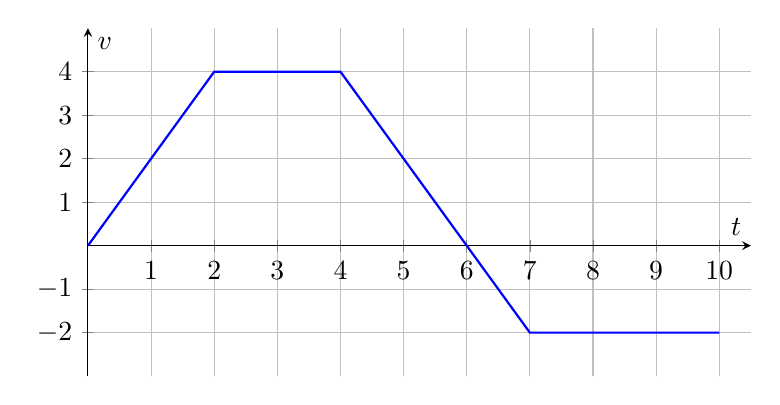
\begin{tikzpicture}
\begin{axis}[width=10cm, height=6cm, xmin=0, xmax=10.5, ymin=-3, ymax=5, axis lines=middle, grid=major, xtick={0,...,10}, ytick={-2,...,4}, xlabel={$t$}, ylabel={$v$}]
    \addplot[blue, thick] coordinates {(0,0) (2,4) (4,4) (7,-2) (10,-2)};
\end{axis}
\end{tikzpicture}
\end{center}
        \begin{enumerate}
            \item What is the displacement of the particle from $t=0$ to $t=10$?
            \item What is the total distance traveled from $t=0$ to $t=10$?
            \item If the particle is at $x=3$ m at $t=0$, where is it at $t=10$?
            \item What is the acceleration at $t=5$? When is the particle farthest from where it started?
        \end{enumerate}
    \end{enumerate}

    \newpage

\item Fundamental Theorem of Calculus, Part 1. Find the derivative.
    \begin{enumerate}
        \item $g(x) = \int_1^x \sqrt{t^3+2}\, dt$
        \item $g(x) = \int_{x^2}^4 t\sqrt{1+t^2}\, dt$
        \item $F(x) = \int_0^{\tan x} \sqrt{1+t^2}\, dt$ for $-\frac{\pi}{2} < x < \frac{\pi}{2}$ (simplify)
        \item $g(x) = \int_{2x}^{x^3} \frac{1}{1+t^4} dt$
        \item Let $g(x) = \int_0^x f(t) dt$, where $f$ is graphed below. Find $g(4)$, $g'(4)$, and $g''(4)$. Where on $[0,6]$ does $g$ have its maximum?

\begin{center}
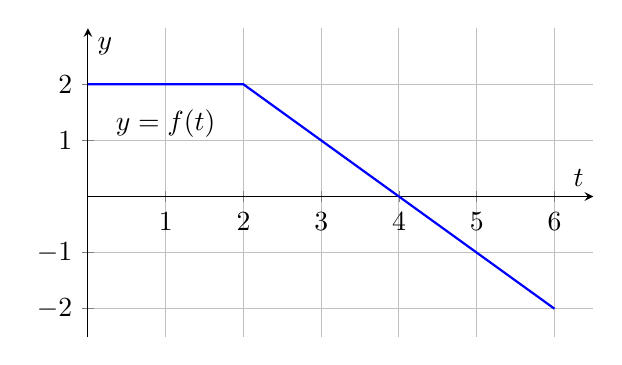
\begin{tikzpicture}
\begin{axis}[width=8cm, height=5.5cm, xmin=0, xmax=6.5, ymin=-2.5, ymax=3, axis lines=middle, grid=major, xtick={0,...,6}, ytick={-2,...,2}, xlabel={$t$}, ylabel={$y$}]
    \addplot[blue, thick] coordinates {(0,2) (2,2) (6,-2)};
    \node at (axis cs:1,1.3) {$y=f(t)$};
\end{axis}
\end{tikzpicture}
\end{center}
    \end{enumerate}

\item Fundamental Theorem of Calculus, Part 2. Evaluate the integral.
    \begin{enumerate}
        \item $\int_1^4 \parens{3\sqrt{x} - \frac{2}{x^2}} dx$
        \item $\int_0^{\pi/4} \sec x \tan x\, dx$
        \item $\int_0^{\pi} (\sin x + 2\cos x) dx$
        \item What is wrong with the calculation $\int_{-1}^2 \frac{1}{x^2} dx = \brac{-\frac{1}{x}}_{-1}^2 = -\frac{3}{2}$?
    \end{enumerate}

    \newpage

\item Substitution. Clearly declare each substitution. For definite integrals, change the bounds to $u$-bounds.
    \begin{enumerate}
        \item $\int \sec^2 x \tan^3 x\, dx$
        \item $\int_0^{\pi/2} \cos x\sqrt{1 + 3\sin x}\, dx$
        \item $\int \sqrt{x}\, \sin\parens{x^{3/2}} dx$
        \item $\int_0^4 \frac{x}{\sqrt{x^2+9}} dx$
        \item $\int_{-2}^1 x\sqrt{x+3}\, dx$
        \item $\int_{-\pi/2}^{\pi/2} x^2 \sin x\, dx$ (look for symmetry first)
    \end{enumerate}

\item Area between curves. Sketch the region and find its area.
    \begin{enumerate}
        \item $y = x^2 - 2x$ and $y = x + 4$
        \item $y = \sqrt{x}$ and $y = \frac{x}{3}$. Find the area integrating with respect to $x$, then with respect to $y$.
        \item $y = \sin x$ and $y = \cos x$ for $0 \leq x \leq \frac{\pi}{2}$
    \end{enumerate}

\item Average value.
    \begin{enumerate}
        \item Find the average value of $f(x) = \frac{1}{x^2}$ on $[1,3]$.
        \item Find the average value of $f(x) = x^2$ on $[0,3]$, and find $c$ in $[0,3]$ with $f(c)$ equal to the average value.
    \end{enumerate}

    \newpage

\item Volumes. Sketch the region and a representative slice. Set up an integral for the volume, then evaluate it.
    \begin{enumerate}
        \item Set up, but do not evaluate. (i) The region under $y = \sin x$ for $0 \leq x \leq \pi$, revolved around the line $y = -1$. (ii) The region between $y = x^2$ and $y = 1$, revolved around the line $y = 1$.
        \item The region between $y = x$ and $y = x^2$, revolved around the $x$-axis
        \item The region under $y = \sqrt{x}$ for $0 \leq x \leq 4$, revolved around the $x$-axis
        \item The region between $y = \sqrt{x}$ and $y = x^2$, revolved around the $y$-axis, and then around the line $x = -1$
    \end{enumerate}

\item Work.
    \begin{enumerate}
        \item A spring has natural length 20 cm, and 0.9 J of work stretches it from 20 cm to 26 cm. How much work stretches it from 24 cm to 28 cm? What force holds it at a length of 30 cm?
        \item A spring has natural length 10 cm and spring constant $k$. Find the work $W_1$ to stretch it from 10 cm to 15 cm and the work $W_2$ to stretch it from 15 cm to 20 cm, in terms of $k$. How are $W_1$ and $W_2$ related?
        \item A 10 m chain with mass 2 kg per meter hangs from the top of a building. How much work does it take to pull the whole chain up to the top? Use $g = 9.8\ \text{m}/\text{s}^2$.
        \item A force of $F(x) = \frac{x}{(x^2+1)^2}$ pounds acts on an object $x$ feet from the origin. Find the work done moving the object from $x=0$ to $x=1$.
    \end{enumerate}

\end{enumerate}

\end{document}
